%%
%%  chapter01.tex - Obstacle Detection and Planning for Autonomous Vehicles based on Computer Vision Techniques
%%
%%  Copyright 2014 Néstor Morales <nestor@isaatc.ull.es>
%%
%%  This work is licensed under a Creative Commons Attribution 4.0 International License.
%%

\graphicspath{{./images/chapter01/bmps/}{./images/chapter01/vects/}{./images/chapter01/}}

\chapter{Change Detection For Obstacle Localization In Images}\label{ch:chapter01}

We drive by mind. That is, once we learn the path to go from a point $A$ to another point $B$, we follow that path without almost thinking. Even more, if a person does this way repeatedly and every day, there will come a time in which they will be able to memorize each black spot, traffic light and even each pothole. So it is not strange that we are always surprised with changes in the signals or the sense of a road.

Following this line of thought, we have developed a system in which we make our prototype to remember the environment of a certain road, making it able to detect changes. In our case, the changes in which we are interested are the obstacles in the way of the vehicle, giving it the ability to avoid them or to stop if necessary. This system is based on a dataset with images associated to localization information. These images will be compared with those captured in real time by the on board cameras. Both images will be registered and changes detected, letting us to know the presence of obstacles or other changes that appeared since the stored images were captured.

This is done through the pipeline shown at figure \ref{fig:cp01_pipeline}. First, the database is captured offline. Then, in real time, images are aligned trough a typical image registration pipeline(feature localization, matching of the features between the images, image transformation and resampling). Once the images are aligned, we retrieve the obstacles.

\section{Method}\label{ch:chapter01_01}

In this section, we will describe each of the stages in the pipeline of the application, starting from the database generation and finishing with the detected obstacles.

\begin{figure}[thb]
  \centering
  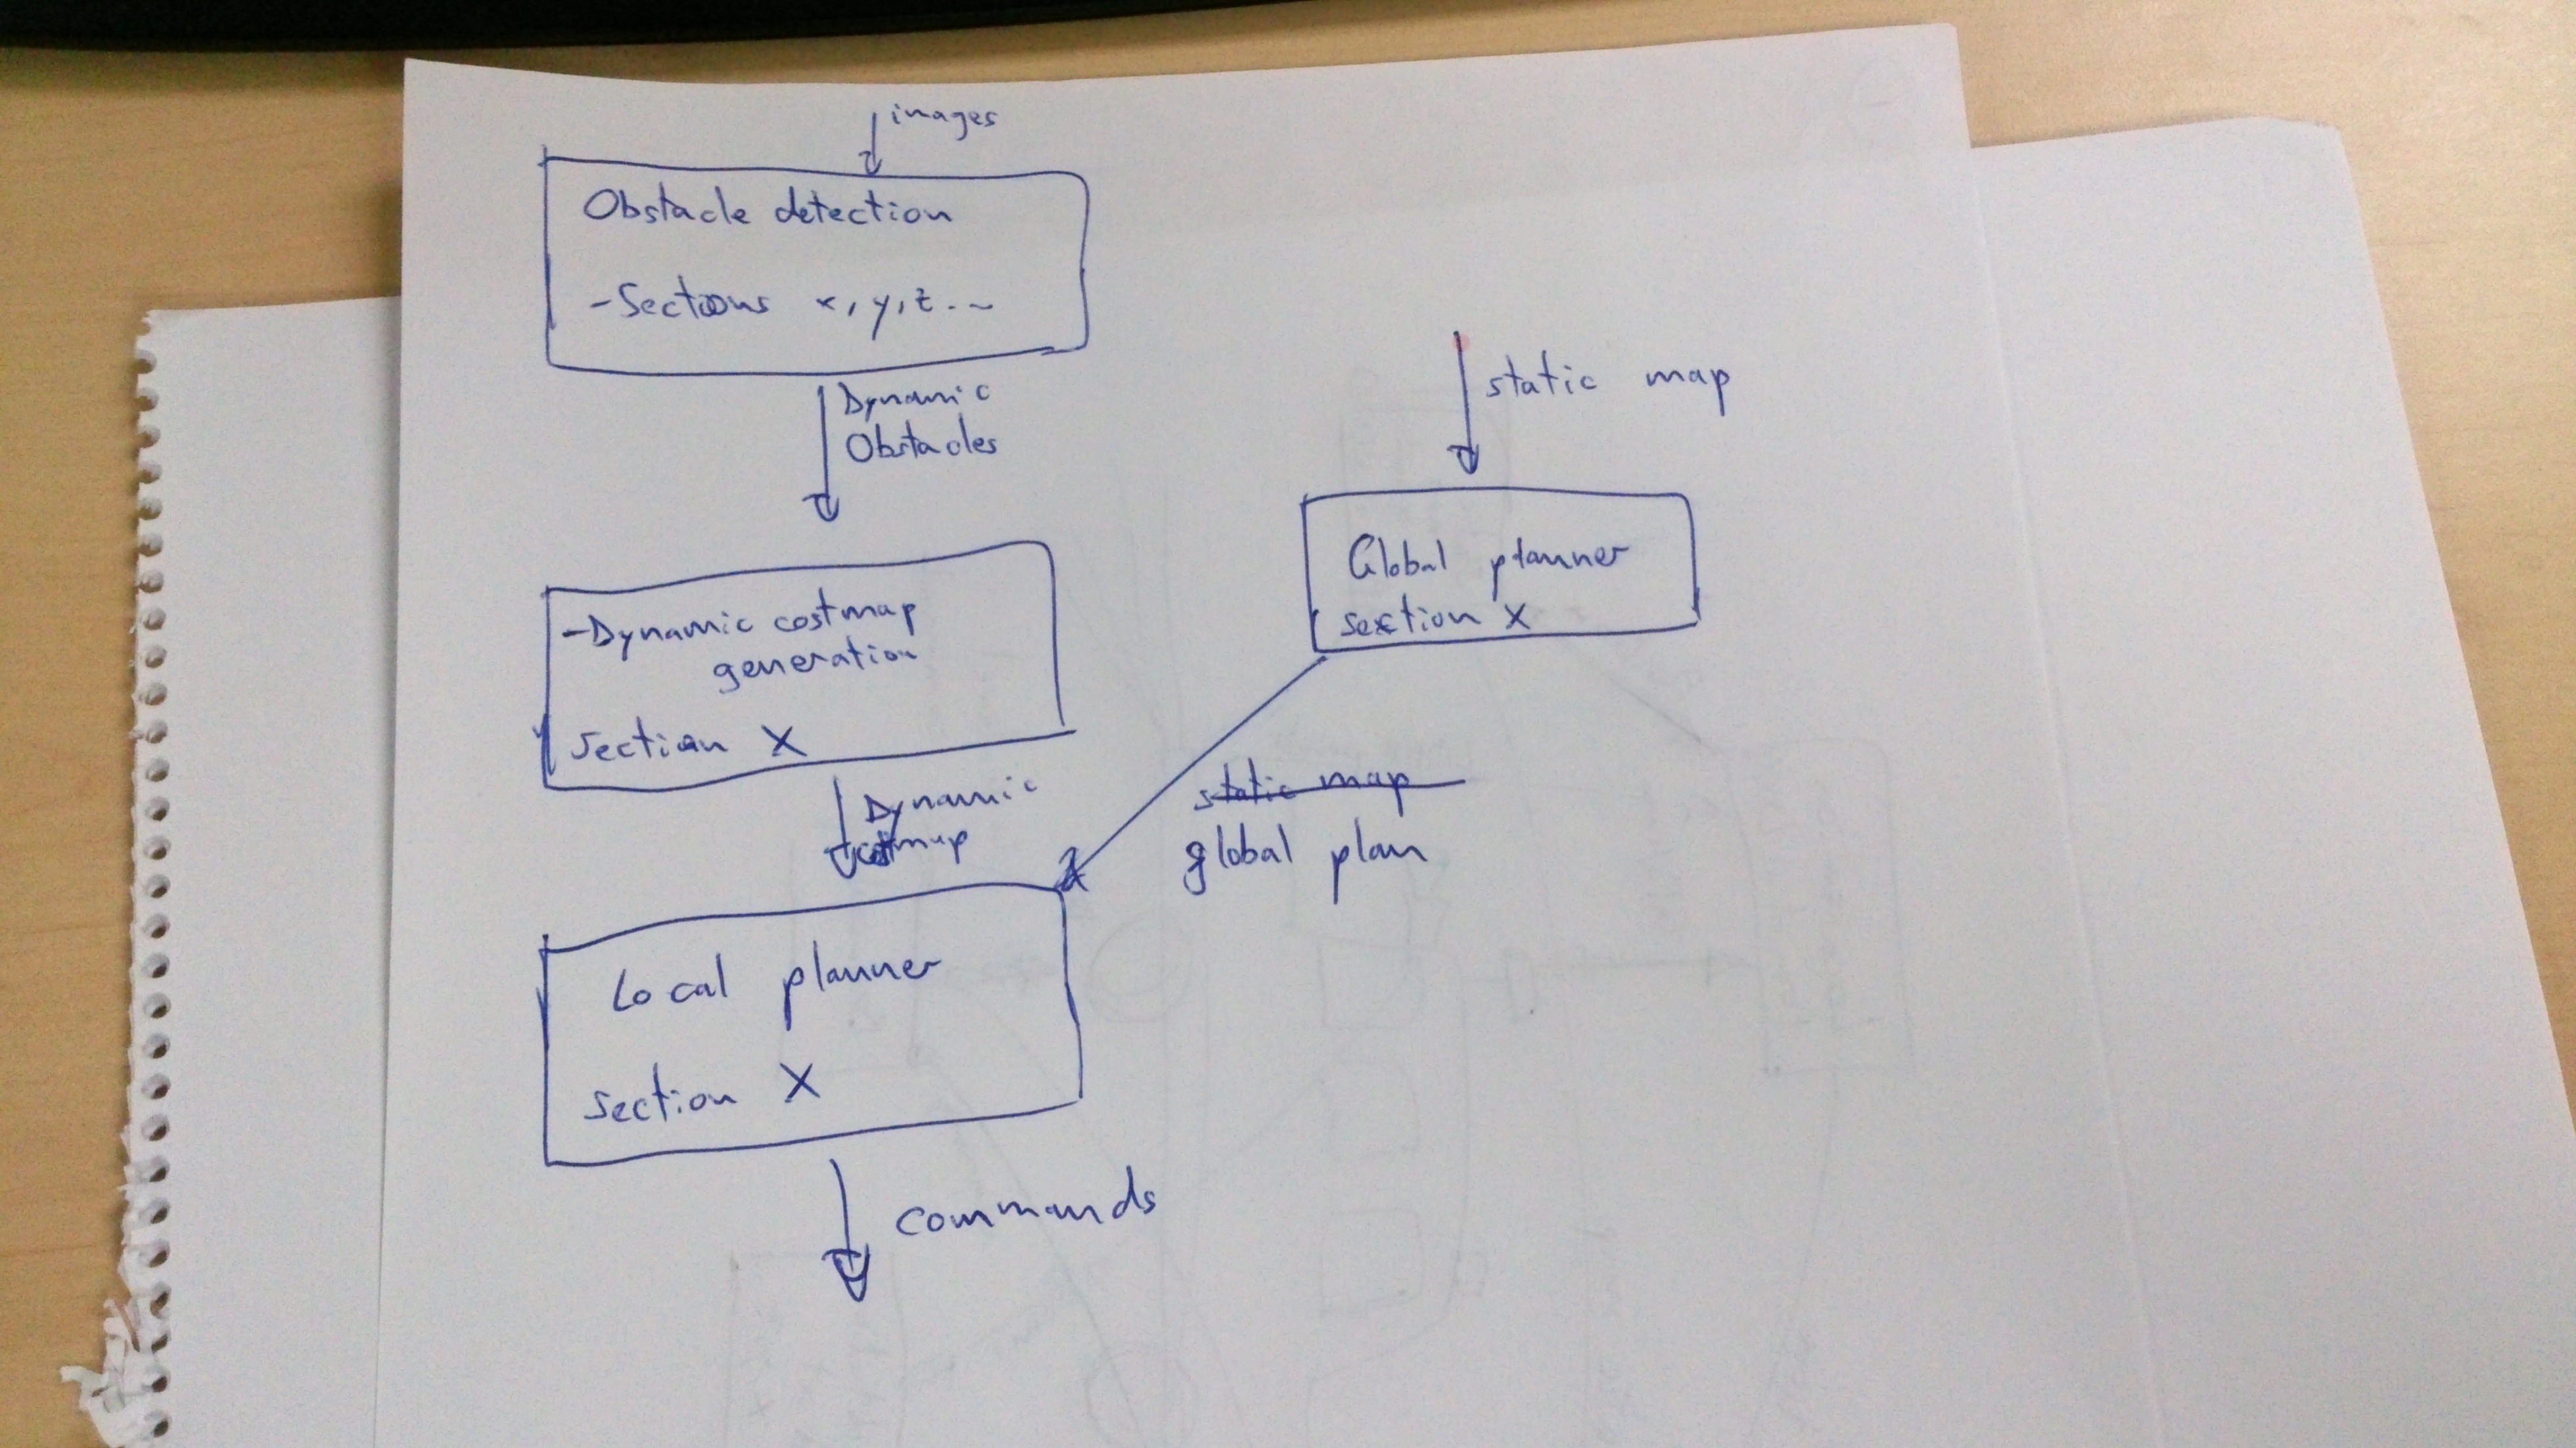
\includegraphics{pipeline}
  \caption{Pipeline of the method.}
  \label{fig:cp01_pipeline}
\end{figure}

As said, the process is based on the generation of an image database in which each image is associated with certain meta-information, being an important part of it the information related to its position in the map, so the first step in the application is the development and population of a database covering the driving area. In this stage, the vehicle will travel inside the covered area, driven by a human or in controlled conditions. While the vehicle is driven, the system stores the set of $320 \times 240$ images, associating geographic information to them: \emph{latitude}, \emph{longitude}, \emph{height} and their transformation into $x$, $y$, $z$ and orientation coordinates with respect to the coordinates frame of the local map. Other information that could be outstanding in the future is also stored (i.e., the day and the hour in which the image was taken, \acs{GPS} rms value, etc.). Images are preprocessed to have as much information as possible, reducing the execution times. For example, we get the set of features from the images offline, not in the real time application. With a $5\,Hz$ update rate, an image is stored about each traveled meter, depending on the speed of the vehicle. In this phase, there should not be any obstacle in the road where the car is going to drive. If so, in the real time execution, fake objects would be detected, due to those obstacles recorded in the database image. Once this process is finished, there will be a database with geographically located images. In figure \ref{fig:cp01_image_database}, a composition of the testing area where some of the stored images have been highlighted is shown.

\begin{figure}[thb]
  \centering
  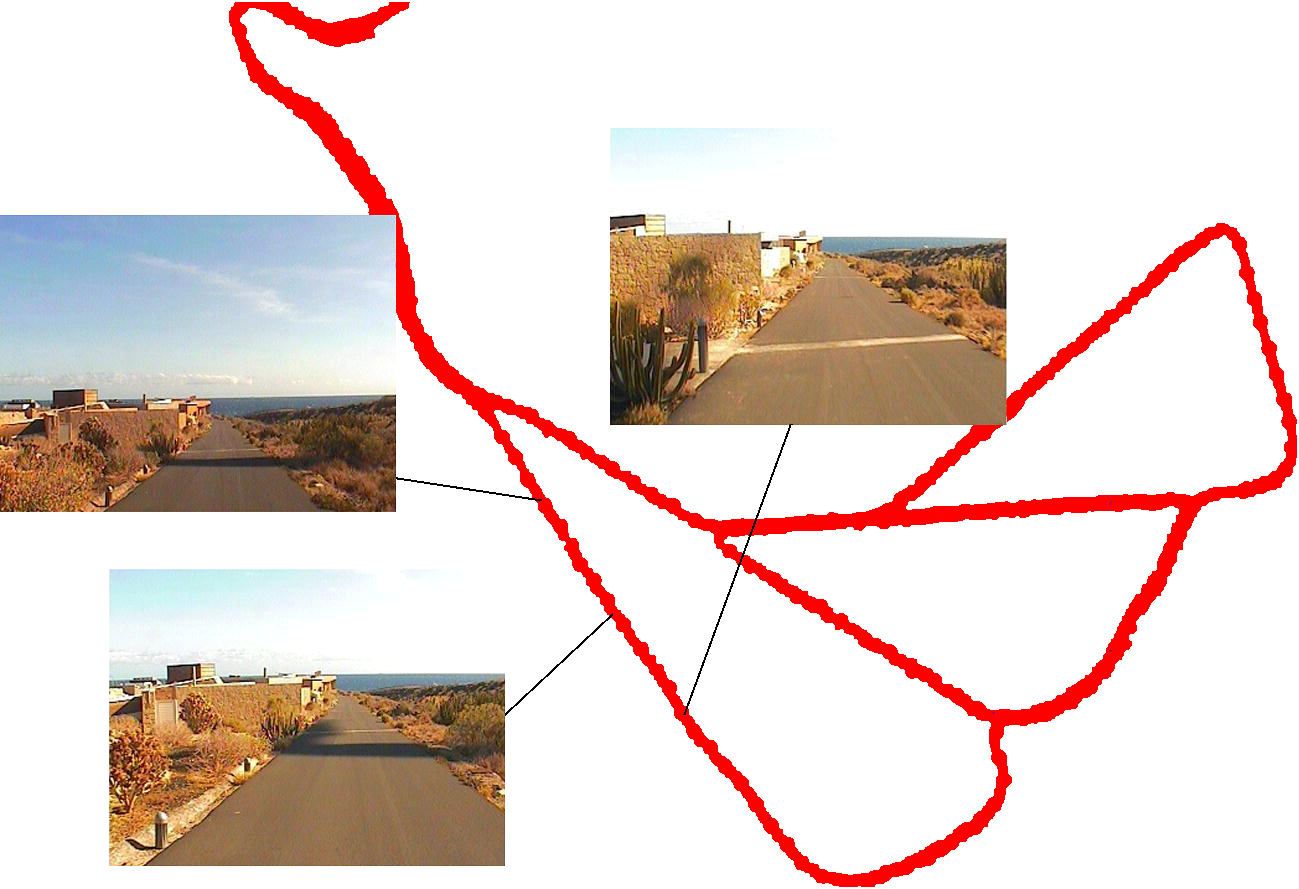
\includegraphics{database}
  \caption{Area covered by the database. Some example images are superimposed.}
  \label{fig:cp01_image_database}
\end{figure}

In real time, the vehicle starts driving by itself. Along the path, it passes over different positions near the recorded route. Positions reported by the \acs{GPS} device are transformed into local coordinates. Simultaneously, an image is obtained from the camera while the nearest image in the database is retrieved. The current frame $I_{RT}$ and the image retrieved from the database $I_{DB}$ are compared by using image change detection techniques, obtaining the obstacles in the scene.

In the moment of the development of this application, localization was entirely retrieved from the \acs{GPS} device. This gave a position each 200 ms, so it was desirable to be able to process each frame under this time. As we will see next, these requirements were finally fulfilled.

\subsection{Image selection from database}\label{ch:chapter01_01_01}

This step will help us to get the most similar image from the database. Most of the times we just need to find an image with the smaller Euclidean distance to the current point, checking that the angular difference is not too big. Although this solution gives good results, many times it is better to have an image not so close to the current point, if that means that all the objects represented in an image are going to appear in the other one. This can be got if an image situated is forward or backward respect to the current image is selected, so one of the images will be contained into the other. Doing that, it will reduce not just the angular difference, but also the lateral distance (which is experimentally the source of most of the misalignments due to an excess of parallax).

In figure \ref{fig:cp01_nearest_image}, we can observe this procedure. Based on this, the nearest image in the database is that obtained by the expression:

\begin{equation}\label{eq:cp01_nearest_image}
I^*_{DB} = \underset{I_{DB}}{\arg\min} \|p_{RT} - p_c\| = {{y_{RT} \cdot v_{DB_x} + x_{RT} \cdot v_{DB_y}} \over 
  {v_{DB_y} \cdot cos(\theta_{RT}) - v_{DB_x} \cdot sin(\theta_{RT})}}
\end{equation}

There, $p_{RT} = (x_{RT}, y_{RT})$ is the position of the vehicle, $p_{DB_i} = (x_{DB_i}, y_{DB_i})$ is the position of each of the images in the database, and $p_c = (x_c, y_c)$ is the crossing point shown at figure \ref{fig:cp01_nearest_image}; $v_{DB_x} = x_{DB} + cos(\theta_{DB})$ and $v_{DB_y} = y_{DB} + sin(\theta_{DB})$; and 
$\theta_{RT}$ and $\theta_{DB_i}$ are the orientations of the vehicle and each of the images in the database. At the end of this selection process a pair of images will be obtained: the current frame ($I_{RT}$), and the associated image extracted from the database ($I_{DB}$). At the same time, we get other related information from the database, like road masks, control points, and other things previously computed.

\begin{figure}[thb]
  \centering
  \includegraphics[trim=0 500 90 90, clip]{nearestImage}
  \caption{Nearest image is retrieved.}
  \label{fig:cp01_nearest_image}
\end{figure}

With the aforementioned method for image selection, we ensure that the image content will be similar in both images based on their geographical associated points. However, as it will be seen in the next sections, the methods employed for the adjustment and comparison of these images are sensitive to illumination changes or other problems caused by shadows or different atmospheric conditions. For this purpose, some extra values are included into the database. These values are the date and the hour in which the image was taken.

Using this information, it is possible to limit the number of images to those in which the external conditions are similar to the current. That is, during the day, the sun is moving and causing different shadows and lights at different times of the day. Different shadows can be considered as fake obstacles by the algorithm, so it is desirable to compare just images in which shadows are similar. Also changes in the brightness of the images could affect to the detection and matching of similar features in both images. To avoid this, just the images in the set $A$ are eligible:

\begin{equation}\label{eq:cp01_eligible_images_by_time}
A = \{ \forall I_{DB} ~|~ \Delta ToD(I_{DB}, I_{RT}) < \tau_{ToD} \wedge \Delta DoY(I_{DB}, I_{RT}) < \tau_{DoY} \}
\end{equation}

, where $I_{DB}$ is each of the retrievable images from the database; $\Delta ToD(I_1, I_2)$ is a function that retrieves the difference in seconds of the \emph{Time of the Day} in which images $I_1$ and $I_2$ were captured; $\Delta DoY(I_1, I_2)$ is a function that retrieves the difference in days of the \emph{Day of the Year} in which images $I_1$ and $I_2$ were captured (we ensure that we are using images taken in similar seasons of the year, and similar lighting conditions). $\tau_{ToD}$ and $\tau_{DoY}$ are free parameters that limit the size of the set $A$.

However, despite of the fact that for most of the cases selecting reference images inside the $A$ set is enough to ensure a good behavior of the method, we can be more restrictive. Even with the selection presented in $A$, illumination can be different in many cases. To minimize this, there is another parameter, the brightness, which is precomputed and stored in the database for a fast retrieval. With this parameter, just images inside the following set will be retrieved:

\begin{equation}\label{eq:cp01_eligible_images_by_brightness}
B = \{ \forall I_{DB} ~|~ \| \mu_{RT} - \mu_{DB} \| < \tau_{\mu} \}
\end{equation}

, where $\mu_{RT}$ and $\mu_{DB}$ are the brightness values for the current image $I_{RT}$ and the database image $I_{DB}$, and $\tau_{\mu}$ is a user defined parameter that limits the size of set $B$. Experimentally, best results are obtained when $\tau_{\mu}$ is below 20\%. An study of the influence of this threshold is presented at section \ref{ch:chapter01_02_01}. Finally, from $A$ and $B$ we get the group

\begin{equation}\label{eq:cp01_eligible_images}
C = A \cap B
\end{equation}

, which will be the input set of images in the retrieval process. $\tau_{DoY}$ and $\tau_{\mu}$ are interrelated. That is, it is needed to have enough images in the set $A$ in order to be sure that $C \neq \emptyset$ after doing the intersection with $B$. To ensure that, images from different days should be chosen in order to guarantee that we find an image with similar illumination conditions to the current frame in the surroundings of the vehicle.

\subsection{Image registration}\label{ch:chapter01_01_02}

In this step, a pair of images which represents the same scene, but taken from different view points, moments and cameras, will be aligned.

This kind of techniques are well known and very used for a big quantity of tasks, like multi-spectral classification, change detection, image stitching, etc., as reflected at \cite{kooper2011stitching, singh1996digital, coppin1996digital, radke2005image, zitova2003image}.

In general, registration techniques have problems with image disparities due to the movement of non static objects (windmills, flags, etc.). Other problems are caused by shadows or reflections that are different depending on the position of the light source (for example, Sun's position during day for images taken out of a building). Quality of the registration also depends on the point of view from where images where taken, or changes in objects in the time course (like a fruit that gets rotten or a bush flowering). All these changes can produce problems depending on the features that are expected to be detected.

Most of the registration methods are composed by the following pipeline: feature detection, feature matching, transformation model estimation, and image resampling and transformation. Same steps have been used in our method.

\subsubsection{Feature detection}\label{ch:chapter01_01_02_01}

First step consists on the detection of similar features in both images, so we will be able to match them in the next step. Therefore, for the same scene, we need the detected features in one image and in the other to be similar, regardless of the effect of perspective, rotation, hidden objects or brightness and contrast changes. One of the first things we must decide is which kind of features will be used, being the most used the features based on corners, borders and areas \citep{li2008comprehensive}. To develop this method, some tests have been made with corners and area based methods. After these tests, results obtained with both corners and region detectors were not discriminative. However, a bigger set of features were detected with corner detectors. But the main difference between both methods is related to the computation time required by each method, requiring more than a second for area based methods.

\paragraph{Corner based methods}\label{ch:chapter01_01_02_01_01}

We refer as corner features those points in which the intensity changes at the image are high in all directions. Since \cite{hans1977towards} made his corner detection operator, a lot of them have appeared like that made by \cite{harris1988combined}, \cite{smith1997susan} (SUSAN), or, more recently, the method used by \cite{rosten2006machine}. Some of these operators have been advanced or modified to improve some characteristics, like the modification of the Harris method made by \cite{shi1994good}.

These operators are, a priori, good enough to be used for this application. However, there are some requirements that the operator must fulfill. First of them is a high detection rate, so the estimation of transformation model that will be used for the adjustment between images will be better. Moreover, once the matching between the features detected in both images is performed, all these points for which a match could not be found will be rejected. Therefore, for a bigger initial dataset, there will be a bigger probability of finding a good number of valid matches. This will allow a bigger set of starting points. Another characteristic that was interesting for this application is to find a high repeatability rate in the detected features. As it will be shown later, it was not so important for the final version of the algorithm due to the matching strategy finally chosen. That allows ensuring with a bigger certainty that we will get correct matches. Finally, last factor that was specially considered was the execution time of the method. This point is specially important because the algorithm must be able to work in real time. This is the first step of the pipeline. If it is too slow, there will not be enough time for other stages. Taking the comparatives performed at \cite{mohanna2001performance, zheng1999analysis} into account, Harris operator shows a higher detection rate, and also a high repeatability rate, with a good performance for affine transformations. It has also a good localization in L-junctions, as well as an acceptable robustness to noise. The weak spot of this operator is that it needs too much resources to calculate the features, which could affect to the final performance. Even so, experimentally the times were not so big to get a bad performance, in special if it is compared, as we will see, with the timings obtained with other methods based in regions like SIFT \citep{lowe1999object} or SURF \citep{bay2008speeded}.

\cite{shi1994good} proposed a method based on \cite{harris1988combined}. In \cite{harris1988combined}, matrix $A$, described at equation \ref{eq:cp01_harris_matrix} is computed for each pixel in the image. From it, the matrix Eigen values $\lambda_1$ and $\lambda_2$ are calculated, which indicates the main curvature of $A$. Based on these, Harris decides if a point belongs to an edge, if it is in a uniform intensity region or if the pixel is a corner.

\begin{equation}\label{eq:cp01_harris_matrix}
A = \nabla I \bigotimes \nabla I = 
\left [ \begin{array}{c} I_x \\ I_y \end{array} \right ]
\left [ \begin{array}{c} I_x \\ I_y \end{array} \right ]^T = 
\left [ \begin{array}{cc} 
I_x^2 & I_xI_y \\ 
I_yI_x & I_y^2
\end{array} \right ]
\end{equation}

, where:

\begin{itemize}
 \item $\nabla = \vec{i} (\partial / \partial x) + \vec{j} (\partial / \partial y)$.
 \item $\bigotimes$ is the outer product.
 \item $I$ is the processed image.
 \item $I_x = {{\partial I} \over {\partial x}}$.
 \item $I_y = {{\partial I} \over {\partial y}}$.
\end{itemize}

\begin{figure*}[h!]
        \centering
        \begin{subfigure}[b]{0.45\textwidth}
                \centering
                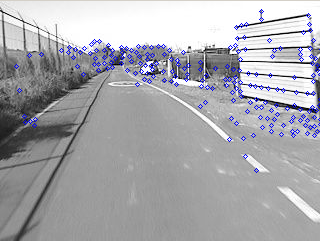
\includegraphics[width=\textwidth]{featuresShi1}
                \caption{$I_{DB}$}\label{fig:cp01_features_shi_1}
        \end{subfigure}%        
        ~ %add desired spacing between images, e. g. ~, \quad, \qquad etc.
          %(or a blank line to force the subfigure onto a new line)
        \begin{subfigure}[b]{0.45\textwidth}
                \centering
                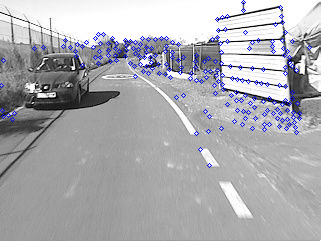
\includegraphics[width=\textwidth]{featuresShi2}
                \caption{$I_{RT}$}\label{fig:cp01_features_shi_2}
        \end{subfigure}%
        \caption{Result of applying the \cite{shi1994good} method over an image pair. The detected corners are similar in both images.}\label{fig:cp01_shi_tomasi_features}
\end{figure*}

To reduce the computational complexity, Harris replaces the use of the Eigen values by the indicator $m_h = det(A) − k \cdot tr^2(A)$, where $k$ is an adjustment parameter and $m_h$ can be considered as a measure of the corner response. To improve this, the method proposed by \cite{shi1994good} uses the smaller of the Eigen values as indicator, instead of $m_h$. This strategy is enough, and in some cases it gives better results than the original operator proposed by \cite{harris1988combined} using less computational time. This is the motive because the \cite{shi1994good} method has been finally used as operator for the detection of the features. In figure \ref{fig:cp01_shi_tomasi_features} we can observe an example of two images, in which the detected features are shown for the \cite{shi1994good} method. One of them was taken from the database $I_{DB}$ (left) and the other is the current image $I_{RT}$ (right).

\paragraph{Area based methods}\label{ch:chapter01_01_02_01_02}

\begin{figure*}[h!]
        \centering
        \begin{subfigure}[b]{0.45\textwidth}
                \centering
                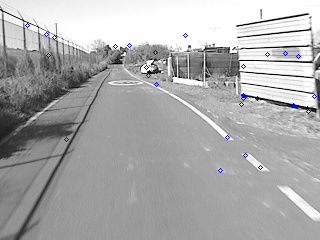
\includegraphics[width=\textwidth]{featuresSIFT1}
                \caption{$I_{DB}$}\label{fig:cp01_features_sift_1}
        \end{subfigure}%        
        ~ %add desired spacing between images, e. g. ~, \quad, \qquad etc.
          %(or a blank line to force the subfigure onto a new line)
        \begin{subfigure}[b]{0.45\textwidth}
                \centering
                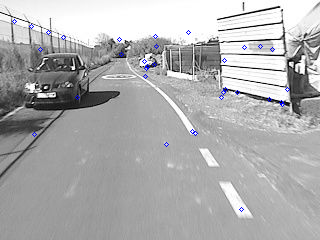
\includegraphics[width=\textwidth]{featuresSIFT2}
                \caption{$I_{RT}$}\label{fig:cp01_features_sift_2}
        \end{subfigure}%
        \caption{Result of applying the \cite{lowe1999object} method over an image pair. The number of detected features is quite smaller.}\label{fig:cp01_sift_features}
\end{figure*}

There are a lot of area based feature detection methods, as well as a lot of reviews, like those presented at \cite{mikolajczyk2005comparison, li2008comprehensive}. Some examples are the region detector of Harris-Laplace, Harris affine and Hessian affine detectors presented by \cite{mikolajczyk2004scale}, the MSER detector proposed by \cite{matas2004robust}, SIFT \citep{lowe1999object} and SURF \citep{bay2008speeded}, among others. Some of these methods, like SIFT or SURF, were tested. In figure \ref{fig:cp01_sift_features} the result of applying the SIFT method to a pair of images is shown. At a first glance, we can observe that although most of the points detected are in the same position in both images, the number of points detected is considerably smaller than these obtained with \cite{shi1994good}. However, the main disadvantage is that the time needed to compute them is too big for the application requirements, and always bigger than the time needed to detect the features with \cite{shi1994good}.

To illustrate this fact, some tests have been performed to obtain a comparison of the computation time needed for \cite{harris1988combined} and \cite{shi1994good} against the time needed by \cite{bay2008speeded} (including feature matching). These times are represented in the chart shown at figure \ref{fig:cp01_features_time_comparison}. It is easy to appreciate that the time needed by \cite{bay2008speeded} is quite bigger than that used by the other corner based methods. In the other hand, the \cite{shi1994good} implementation seems to be slower than \cite{harris1988combined}, but the experimental tests showed that the final algorithm gave better results in obstacle detection terms when the first one was used, and time difference is not so big. So it was the finally chosen method as feature detector.

\begin{figure}[h!]
\centering
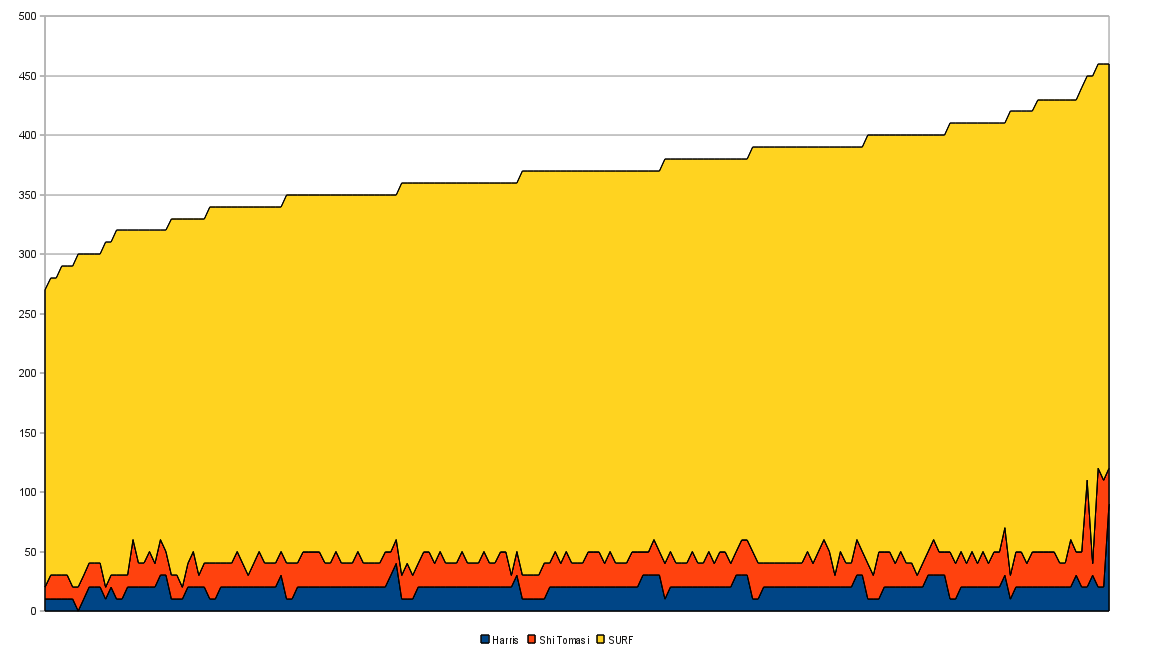
\includegraphics{featuresTimeComparison}
\caption{Timing results after the comparison of the different feature detection methods, including their matching.}\label{fig:cp01_features_time_comparison}
\end{figure}

\subsubsection{Feature matching}\label{ch:chapter01_01_02_02}

Once the features have been detected in both images, next step is matching them. In a preliminary version of the algorithm, we tried to do the match directly using methods like \acf{NCC} or similar, since the computation of descriptors of the surrounding area of each feature could be too expensive. In the final version of the algorithm, we just detect points in one of the images because optical flow methods will be used to detect the correspondences within the second image. This is the motive because the repeatability characteristic in the feature detectors was not so important at the end.

We detect the features in the image $I_{DB}$, because it allows calculating these features offline. This will reduce the computation time of the algorithm. We decided to use sparse optical flow methods, also for optimization reasons.

The method chosen to perform the optical flow is that proposed by \cite{lucas1981iterative}. This method, quite known and contrasted, gives excellent results when the difference between the images is not too big. However, when this difference is increased, results are worthier, which has forced us to have a bigger window and, consequently, bigger computational time requirements. Because of that, we need to use the pyramidal implementation proposed by \cite{bouguet2001pyramidal}. This method will allow locating points with a big distance between them, while ensuring good results.

\cite{bouguet2001pyramidal} method produces a significant improvement in the results, but there still are bad matched points. To minimize this effect, we perform a double-check as follows: from a set of points $S_1$ selected from the image retrieved from the database, the point set $S_2$ is located by using optical flow techniques from $I_{DB}$ to $I_{RT}$. Once this second set is calculated, the optical flow is performed from the points in the set $S_2$ in $I_{RT}$ to $I_{DB}$, obtaining the point set $S_3$. All the points that are in the intersection of $S_1$ and $S_3$ will be considered as valid. The others will be rejected. That is,

\begin{equation}\label{eq:cp01_rejected_points}
P_{final} = \{ p_i ~|~ p_i \in S_1 \cap S_3 \}
\end{equation}

An example of the matches obtained with this method is shown at figure \ref{fig:cp01_matches}. There, the points with a similar color represent a match.

\begin{figure*}[h!]
        \centering
        \begin{subfigure}[b]{0.45\textwidth}
                \centering
                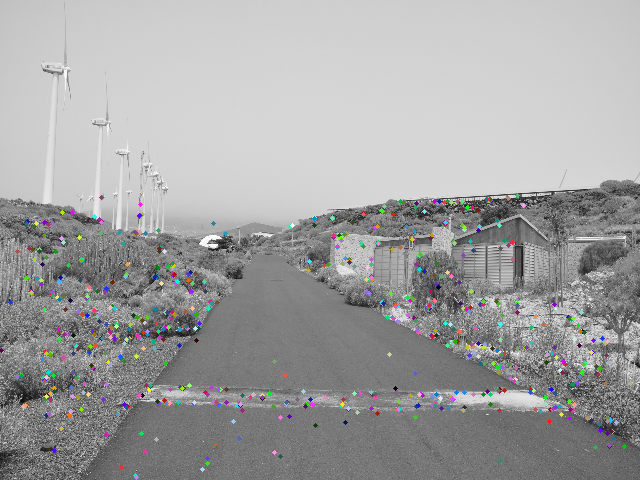
\includegraphics[width=\textwidth]{matches1}
                \caption{$I_{DB}$}\label{fig:cp01_matches_1}
        \end{subfigure}%        
        ~ %add desired spacing between images, e. g. ~, \quad, \qquad etc.
          %(or a blank line to force the subfigure onto a new line)
        \begin{subfigure}[b]{0.45\textwidth}
                \centering
                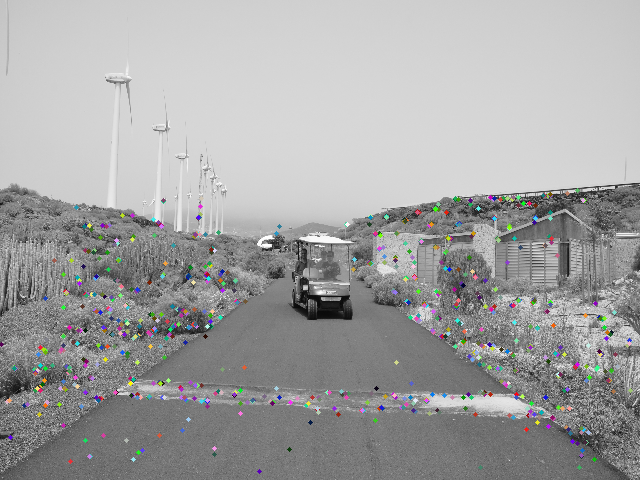
\includegraphics[width=\textwidth]{matches2}
                \caption{$I_{RT}$}\label{fig:cp01_matches_2}
        \end{subfigure}%
        \caption{Correspondences between points. Each color represents a match.}\label{fig:cp01_matches}
\end{figure*}

\subsubsection{Transform model estimation}\label{ch:chapter01_01_02_03}

The final objective of any image registration algorithm is to transform an image into another. In most of the applications in which the perspective warp is not too strong, just global mapping techniques are needed. Some examples where global mapping is enough are the affine transformations for satellite images, or projective transformations for aerial images, which are slightly more affected by perspective.

For this application, global methods do not provide good results, since the images are locally warped. Then local mapping models are a better choice. Global mappings are insufficient as there are objects in first and second plane, a strong perspective warping and different points of view. In different sources it is possible to observe the superiority of local mapping models against global mapping models at certain circumstances, as seen at \cite{goshtasby1988image, ehlers1994high, wiemker1996application, flusser1992adaptive}.

In order to select the most suitable mapping model, some non-rigid transformation functions have been tested. In particular, the preselected methods for the comparison are \ac{TPS} \citep{harder1972interpolation}, \ac{WM} \citep{goshtasby1993design} and \ac{PL} \citep{goshtasby1986piecewise}. As one of the most critical parameters of the method is the timing, the time needed by each of the three methods for different numbers of point pairs has been measured. In figure \ref{fig:cp01_transform_model_time}, these times are represented for each of the tested functions.

\begin{figure}[h!]
\centering
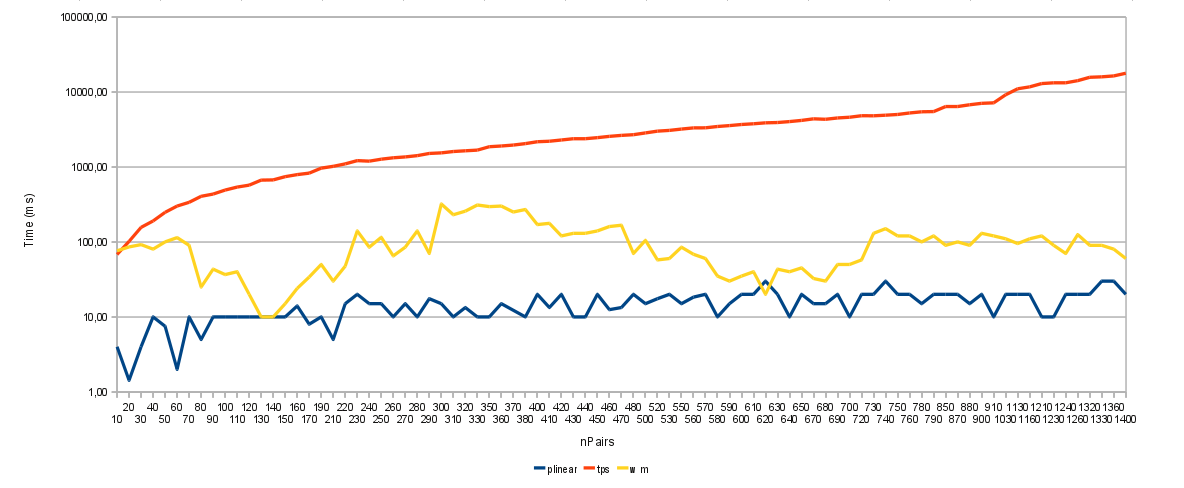
\includegraphics[width=\textwidth]{compTransf}
\caption{Comparison of three possible methods for non-rigid image transform.}\label{fig:cp01_transform_model_time}
\end{figure}

As seen, \ac{TPS} function is by far the most time-consuming from all of them, giving poor results also with a small number of points. This is because for this transformation, in the first instance a system of $N + 3$ linear equations must be solved, which requires about $N^2$ multiplications (being $N$ the number of point pairs). Also, TPS is a kind of global method, so it uses all $N$ correspondences, giving a total of $n^2N$ operations (supposing an image of size $n \times n$). Knowing this, the total computational complexity of the TPS method is $\mathcal{O}(N^2) + \mathcal{O}(n^2N)$ \citep{zagorchev2006comparative}. If this computational complexity is compared to that of \ac{WM} ($\mathcal{O}(n^2N)$) or \ac{PL} ($\mathcal{O}(N~log(N)) + \mathcal{O}(n^2)$), then it is easy to understand why these times are so bigger. In the \acf{WM} method, the coefficients of the weight functions are the same as the coordinates of the feature pairs, so there is no computational time involved in its calculations, as happened for the \ac{TPS} method. However, coordinates of all points are used in the calculations, so the mapping of each pixel needs $N$ multiplications.

In the other hand, \acf{PL} is composed by two different stages. In the first one, triangles must be generated and a transformation between the corresponding triangles calculated, which requires about $N~log(N)$ comparisons. Once the triangles have been generated, the transformation for each pixel needs a small number of operations ($\mathcal{O}(n^2)$).

In the chart shown at figure \ref{fig:cp01_transform_model_time}, it is shown that there is not a very big difference between the times obtained by the Weighted Mean and Piecewise Linear methods. In some special cases, even the times of Weighted Mean are better than those obtained by \ac{PL}. Anyway, results are better for the Piecewise Linear algorithm and they are just in the limit the method can afford, if we take into account the times required by the previous stages of the algorithm (more information about the timings of the different parts of the full method is provided in section \ref{ch:chapter01_02_03}). As \ac{WM} is computationally more expensive, we discarded it to ensure a fast execution.

In general, Piecewise Linear presents some problems if not so many points are paired, which can originate big triangles and a bad local registration, especially in presence of bad paired points. In the problem being solved here, just the obstacles in the road will be detected. This fact solves part of the problem of the bad warped images (This is better explained at section \ref{ch:chapter01_01_03_03}). However, when part of the image appears inside of the road due to a bad transformation, fake obstacles will be detected. There is no way to solve this with the used techniques, and using other methods will produce bad timing results. But this problem will appear in just one frame at once, so in the next frame the fake obstacle will be rejected.

In the first step of the piecewise linear method, a Delaunay’s triangulation is performed based on the control points calculated in the previous steps. This method ensures that the circumcircle of any obtained triangle is not going to contain any vertex of another triangle. In figure \ref{fig:cp01_triangulation} we observe the result of performing the triangulation over the points calculated for the images shown before.

\begin{figure*}[h!]
        \centering
        \begin{subfigure}[b]{0.45\textwidth}
                \centering
                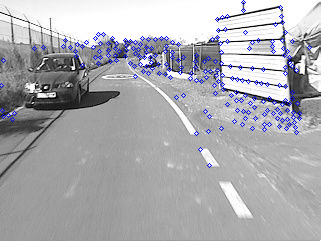
\includegraphics[width=\textwidth]{triangulation1}
                \caption{Initial points.}\label{fig:cp01_triangulation_1}
        \end{subfigure}%        
        ~ %add desired spacing between images, e. g. ~, \quad, \qquad etc.
          %(or a blank line to force the subfigure onto a new line)
        \begin{subfigure}[b]{0.45\textwidth}
                \centering
                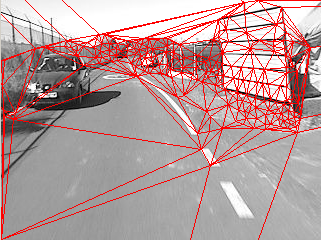
\includegraphics[width=\textwidth]{triangulation2}
                \caption{Delaunay triangulation.}\label{fig:cp01_triangulation_2}
        \end{subfigure}%
        \caption{Original points and the obtained triangulation.}\label{fig:cp01_triangulation}
\end{figure*}

Vertexes of the obtained triangles allow defining other triangles in the second image, since the correspondence of all the points in both images is known. The idea is that, given the coordinates of three control points (vertex of a triangle), and their correspondences in the other image ($[(X_1, Y_1), (x_1, y_1)]$, $[(X_2, Y_2), (x_2, y_2)]$, and $[(X_3, Y_3), (x_3, y_3)]$), it is desired to determine the linear mapping functions $X = f(x, y)$ and $Y = g(x, y)$. These functions will transform a triangle of the first image into the corresponding triangle in the second image. In other words, given three three-dimensional points $(x_1, y_1, X_1)$, $(x_2, y_2, X_2)$, and $(x_3, y_3, X_3)$, the parameters of the plane $X = f(x, y)$, which pass over these points, will be calculated. The same process is done for the $Y$ plane.

The same procedure will be performed for all the pixels $(x_i, y_j)$ of the image $I_{DB}$, which will be transformed. Pixels that represent the same surface in the real world will be aligned having the same position in both images. We do not want to warp the obstacles, so we transform the image $I_{DB}$, which is free of obstacles.

\subsubsection{Image resampling and transformation}\label{ch:chapter01_01_02_04}

In the previous stage a new position has been defined for each pixel in the original image. In this step, we just calculate, for each new position of the pixel in the image $I_{DB}$, the appropriate value of the color components by interpolation. For that, the color in the neighborhood of the pixel in the initial position at the original image is used, in order to get a soft image without strong changes which would distort the final result. The most common techniques, like the nearest neighbor, bilinear and bicubic interpolation have been tested, obtaining the best results with the bicubic interpolation. The result of the resampling process is shown at figure \ref{fig:cp01_transform_and_resample}.

\begin{figure}[h!]
\centering
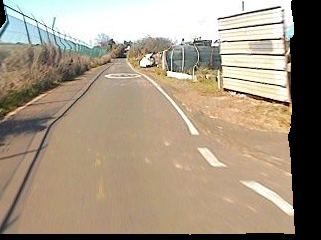
\includegraphics[width=0.45\textwidth]{transformed}
\caption{Resulting transformed image.}\label{fig:cp01_transform_and_resample}
\end{figure}

\subsection{Obstacle detection}\label{ch:chapter01_01_03}

The detection of the obstacles is performed in three different steps: mask generation, the obstacle detection itself, and a selection of the finally considered obstacles.

\subsubsection{Mask generation by using Delaunay triangulation algorithm}\label{ch:chapter01_01_03_01}

Using the Piecewise Linear method, mapping just can be done inside the region occupied by the obtained triangles. Outside of them, mapping cannot be done. In many cases, this is enough to detect an obstacle. If a mask that covers all the image subset where the triangles are positioned is created, practically all the image will fall inside this area. This happens when there are points dispersed all around the image, or they are enough dispersed to detect the obstacles because they are inside the covered area. This can be observed at figure \ref{fig:cp01_mask_is_covering}.

\begin{figure*}[t]
        \centering
        \begin{subfigure}[b]{0.45\textwidth}
                \centering
                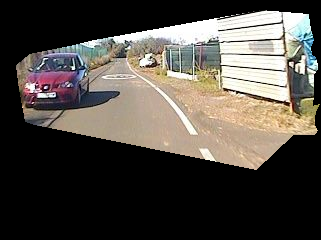
\includegraphics[width=\textwidth]{maskCovers2}
                \caption{The mask covers the obstacle that is going to be detected.}\label{fig:cp01_mask_is_covering}
        \end{subfigure}%        
        ~ %add desired spacing between images, e. g. ~, \quad, \qquad etc.
          %(or a blank line to force the subfigure onto a new line)
        \begin{subfigure}[b]{0.45\textwidth}
                \centering
                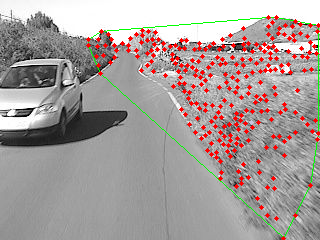
\includegraphics[width=\textwidth]{maskNotCovers}
                \caption{The area covered by points is not enough to detect the obstacle.}\label{fig:cp01_mask_not_covers}
        \end{subfigure}%
        \caption{Mask examples.}\label{fig:cp01_mask_examples}
\end{figure*}

However, in the processed images a big part of the pixels of each image represents the road, which is a soft surface without corners to be detected. Also when an obstacle appears no correspondences can be found, so there are not control points that allow computing the triangulation in those areas. So there are big chances of having a mask that does not cover them, as happens in the example shown at figure \ref{fig:cp01_mask_not_covers}. To solve this, we use a projective transformation which is calculated using the matched points, but just for pixels that are out of the areas covered by these correspondences are transformed using this method. This allows comparing also the areas where there are not matched corners, at the cost of not having the same precision in the transformation as that obtained in the rest of the image, but allowing detecting obstacles also in the not matched area. In general, this happens when an obstacle is very close to the vehicle, so the precision will not be as important as it is quite possible that an obstacle is in this area.

\subsubsection{Obstacle detection}\label{ch:chapter01_01_03_02}

The goal of this algorithm is the detection of the obstacles that are in the road by just using image comparison. As images are now well adjusted, both images can be compared pixel by pixel to detect these differences. A first approach is to make a direct comparison between the pixels by calculating the absolute difference of pixels in both images. If this difference is over a threshold $\tau$, the pixel is considered as part of an obstacle. The problem is that the only way to select the threshold $\tau$ is experimentally. In part due to this, results obtained with this method are not quite good and, mainly, not very robust, so it is needed to find more advanced techniques.

A more robust way to locate these changes is by performing a \ac{PCA}, by creating a bidimensional data set based on the brightness information from both images. The idea is that brightness relation between pixels at the same position in both images will be generally similar, except for those pixels in which the obstacle is represented. In other words, although the color of the elements in one image and the other can be slightly different, the relation between the colors in both images will be approximately constant for all pixels. When this relation differs from that present in the most of pixels, an obstacle is detected. It has to be taken into account that this fact is not always true. When there are different environment conditions, not all materials reflect the light in the same way. This can produce fake obstacles, but we can discriminate later fake obstacles by just selecting those that are inside the road, which is a constant surface where the relation between the pixels should be similar in all the area covered by it.

In that way it is possible to study the main correspondence between the gray levels from an image and the other one, considering as changes the points in which their brightness difference differs from the main trend.

To do that, a set of points $S$ is created.

\begin{equation}\label{eq:cp01_brightness_relation}
S = \{ p(I_1(x, y), I_2(x,y)) ~|~ x \in \{1 \dots W\}, y \in \{1 \dots H\} \}
\end{equation}

, where $W$, $H$ are the width and height of the images; and $I_i(x, y)$ is the brightness value of the image $i$ at point$(x,y)$. Set $S$ is represented in the chart in the left image of figure \ref{fig:cp01_pca}.

After performing the \ac{PCA}, a set $S'$ is obtained from the initial set $S$, which is represented in the central image of figure \ref{fig:cp01_pca}. It can be observed that there is a common trend in the pixels around the line. But there is a cluster of points that are not following this trend, which are far from the line. If the distance of each point is represented at the pixel original position, we get an image like that shown on the right side of the figure. There, brightest points are those with a bigger distance to the line. In other words, having a point $p(I_1(x, y), I_2(x, y))$ in the left chart, the represented value for the point $q(x, y)$ in the generated image will be the smaller distance of the point $p$ to the line shown in the central chart.

\begin{figure}[h!]
\centering
\begin{minipage}{0.3\textwidth}
    \centering
    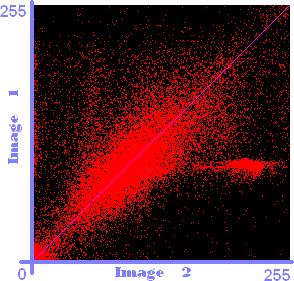
\includegraphics[width=\textwidth]{pca1}\label{fig:cp01_pca1}
\end{minipage}
\begin{minipage}{0.3\textwidth}
    \centering
    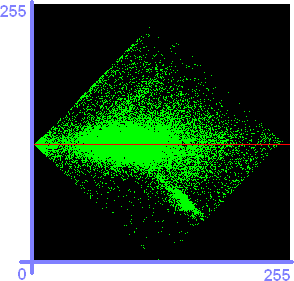
\includegraphics[width=\textwidth]{pca2}\label{fig:cp01_pca2}
\end{minipage}
\begin{minipage}{0.3\textwidth}
    \centering
    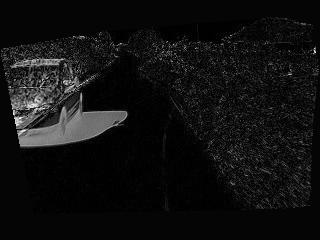
\includegraphics[width=\textwidth]{pca3}\label{fig:cp01_pca3}
\end{minipage}
\caption{Representation of the correspondences of the pixels gray level in both images before ($S$) and after applying PCA ($S’$). On the right, a representation of the distances of all the points in the sensed image is shown.}\label{fig:cp01_pca}
\end{figure}

A threshold that tells if a pixel belongs to an obstacle or not must be chosen, but before applying a threshold, some morphological operations are performed to remove the noise.

By applying the threshold we will get some clusters of pixels that can be considered as obstacles. By using a contour detector these pixel clusters can be grouped into connected areas and reject the areas with a smaller size. In figure \ref{fig:cp01_pipeline_example}, two examples of the pipeline described in this chapter are shown. Also, in figure \ref{fig:cp01_sequence_example}, a set of images represent the detection of a car performed by the method along a sequence recorded in the testing area.

\subsubsection{Selection of the desired obstacles}\label{ch:chapter01_01_03_03}

We are not interested in the obstacles that are outside of the road, as we just need to detect the obstacles that could damage or be damaged by the vehicle, like other vehicles, cyclists, pedestrians, stones, etc. To do that, we need to define a mask that indicates which part of the image belongs to the road. This segmentation is performed over the image stored at the database ($I_{DB}$). This allows segmenting the image offline, expending all the computational time for other tasks.

In order to obtain this mask, the method described by \cite{arnay2009applying} was used. This technique consists on the employment of an \ac{ACO} based algorithm for the detection of roads in unstructured environments. The algorithm assumes that, if the vehicle is on the road, the boundaries of the road are two curves that go from the bottom of the image to the horizon line. The output of this method is a pair of series of pixels, one for each boundary of the road.

In real time, the same transformations aforementioned are applied to the mask to adapt it to the sensed image. By positioning the mask over the detected obstacles, those outside of the road are rejected. We can see the result of this process at figure \ref{fig:cp01_mask_warped}.

\begin{figure}[h!]
\centering
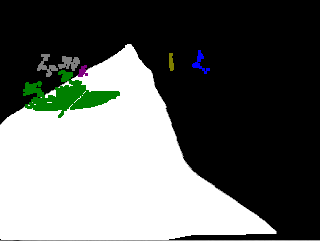
\includegraphics[width=0.45\textwidth]{maskWarped}
\caption{Detected objects on the transformed mask.}\label{fig:cp01_mask_warped}
\end{figure}

\section{Summary}\label{ch:chapter01_03}

The presented algorithm is able to detect the obstacles in the road by integrating three different sensors: a \acs{GPS} device, an \ac{IMU} and a vision system. This algorithm presents an acceptable detection rate, as we will see in the results chapter, in section \ref{ch:chapter01_02}.

The method accomplishes the objectives for which it was designed. It uses image registration techniques to solve the alignment problem, trying to make the simpler use of them, without complex strategies, in order to get a real time execution. This method presents an alternative way to detect obstacles that works correctly and fast and it also could be used in other tasks, specially in video surveillance.

The algorithm is made up by some very different stages which combine image registration and change detection techniques, among others. In the first stage, a complete database of geographically referenced images is created. Then, some methods for the localization of the best images to be used as input for the rest of the algorithm have been implemented and tested, always trying to get the best results. For these images, usual four image registration steps are performed (feature detection, matching, transform model estimation and image resampling and transformation). Many methods have been studied for the development of these tasks, selecting the most suitable. Sometimes good methods had to be rejected due to time limitations, selecting just those methods which gave the best results within acceptable times.

The stages of mask generation, obstacle detection and selection gave good results, avoiding problems like those originated by brightness, contrast or color differences, but not for other problems like shadows or strong changes in the environment. All of this makes it robust and reliable, if the condition of a highly populated database is fulfilled. The method has been fully tested, both with the use of benchmarks, and also in real conditions, which validates the good behavior of the algorithm.

However, this method still suffers from some of the weaknesses described in \ref{ch:chapter01_01}:
\begin{enumerate}
 \item We are still not able to locate the exact position of the obstacles in real world coordinates.
 \item We need a highly populated image database in continuous update, with the maintenance problems related to such a system. If we also consider the need of having images associated to a scene in different illumination and weather conditions, this system becomes really hard to be deployed using the current technology.
 \item We are not tracking the obstacles, so we can not do an intelligent planning taking into account the behavior of the obstacles. 
\end{enumerate}

Anyway, we think that the image registration and change detection steps of the algorithm could be used successfully as improvement of change detection methods in aligned video sequences, like those presented by \cite{diego2011video, evangelidis2011slice, evangelidis2011efficient}. 

In the following chapters, we will see several approaches we tried in order to avoid the weaknesses enumerated. In the next chapter, we will introduce a method in which we isolated the last of them, with the aim of tracking of the obstacles, but without applying serious attempts to locate them in real world coordinates. For that, static images used for the detection of the foreground and a non rigid point set registration algorithm is used.
























